\section*{\centering BAB IV \\ Metode Penelitian}

\addcontentsline{toc}{section}{BAB IV Metode Penelitian}  % Manually add unnumbered section to ToC

% Set the section counter manually to "1" for subsections under BAB IV
\setcounter{section}{4}
\setcounter{table}{0}
\setcounter{subsection}{0}  % Reset subsection
\setcounter{figure}{0}
\renewcommand{\thefigure}{\thesection.\arabic{figure}}
\renewcommand{\thetable}{\thesection.\arabic{table}}

\subsection{Analisis Permasalahan}
KPU Provinsi Lampung saat ini sedang melaksanakan agenda lima tahunan Pilkada. Sebagai bagian dari persiapan Pilkada 2024, KPU Provinsi Lampung telah melakukan rekapitulasi daftar pemilih. Namun, untuk memahami distribusi dan karakteristik daftar pemilih antar kecamatan di 15 Kabupaten Lampung, diperlukan sebuah analisis yang lebih mendalam. Solusi yang diusulkan adalah penerapan teknik klusterisasi pada data rekapitulasi tersebut, serta penggunaan data opsional lain dari BPS untuk memperkaya analisis. Hasil klusterisasi ini diharapkan dapat memberikan wawasan tambahan melalui visualisasi interaktif yang lebih informatif.

\subsection{Alur Penyelesaian}
\begin{figure}[h]
    \centering
    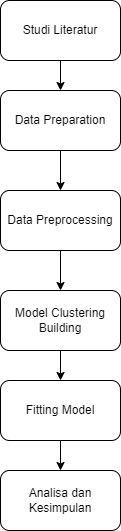
\includegraphics[width=0.2\linewidth, height=10cm]{images/flow.png}
    \caption{Alur Penyelesaian Penelitian}
    \label{fig:flow}
\end{figure}

\subsection{Studi Literatur}
Pada tahap ini, penulis melakukan kajian literatur yang berkaitan dengan klusterisasi data, baik pada data pemilih maupun data umum lainnya. Penelitian yang ada menjadi dasar untuk memilih metode klusterisasi yang tepat dan teknik validasi model. Selain itu, literatur yang mengkaji metode penentuan jumlah cluster optimal, seperti Elbow Method dan Silhouette Score, menjadi acuan dalam menentukan parameter optimal pada penelitian ini.

\subsection{Data Preparation}
Persiapan data (\textit{data preparation}) adalah tahap awal sebelum data dapat digunakan dalam model. Pada tahap ini, data masih dalam bentuk mentah dan belum melalui proses normalisasi. Data yang digunakan pada penelitian ini adalah dataset rekapitulasi daftar pemilih untuk Pilkada 2024 Provinsi Lampung dan data tambahan dari BPS  untuk seluruh Kecamatan di Provinsi Lampung.
\begin{table}[ht]
\centering
\resizebox{\textwidth}{!}{
\begin{tabular}{|l|r|r|r|r|r|r|r|r|}
\hline
\textbf{Sub-Region} & \textbf{Male Voters} & \textbf{Female Voters} & \textbf{Total Voters} & \textbf{Voter Gender Ratio} & \textbf{Total Population} & \textbf{Population Growth Rate (\%)} & \textbf{Population Density} & \textbf{Eligible Voter Ratio} \\ \hline
KEDATON             & 19196                & 19657                 & 38853                & 97.65                      & 52400                    & -0.17                              & 13896                      & 74.146947                      \\ \hline
SUKARAME            & 23913                & 24623                 & 48536                & 97.12                      & 67100                    & 0.65                               & 6148                       & 72.333830                      \\ \hline
TANJUNG KARANG BARAT & 22329                & 22631                 & 44960                & 98.67                      & 63200                    & 0.72                               & 5476                       & 71.139241                      \\ \hline
PANJANG             & 26859                & 26298                 & 53157                & 102.13                     & 74900                    & 0.23                               & 5488                       & 70.970628                      \\ \hline
TANJUNG KARANG TIMUR & 14017                & 14236                 & 28253                & 98.46                      & 38500                    & -0.37                              & 18619                      & 73.384416                      \\ \hline
\end{tabular}
}
\caption{Dataset Rekapitulasi Daftar Pemilih}
\label{tab:method_voter_population_data}
\end{table}


\subsection{Data Preprocessing}
Setelah data terkumpul, dilakukan tahap praproses data (\textit{data preprocessing}). Pada tahap ini, penulis menentukan atribut yang relevan untuk proses klusterisasi dan melakukan normalisasi data guna memastikan keseragaman skala atribut. Tabel \ref{tab:method_voter_population_data} berisikan 230 record baris data rekapitulasi per kecamatan di Provinsi Lampung. Proses normalisasi data dilakukan agar nilai dari setiap variable berada pada rentang yang sama, menghindari pengaruh dominasi fitur tertentu pada model klusterisasi.

\subsubsection{Feature Selection}
Untuk memastikan hasil klusterisasi yang lebih bermakna, dilakukan pemilihan fitur (\textit{feature selection}) terhadap atribut data. Atribut yang dipilih mencakup data demografis seperti usia, jenis kelamin, dan kepadatan populasi, yang dapat memberikan insight terkait pola pemilih di berbagai kecamatan. Atribut-atribut ini ditentukan melalui analisis korelasi untuk menghindari redundansi dan memastikan keterkaitan yang erat dengan tujuan penelitian.
\begin{table}[h]
    \centering
    \label{tab:original_data}
        \resizebox{\textwidth}{!}{
            \begin{tabular}{|l|c|c|c|c|}
        \hline
        \textbf{Sub-Region} & \textbf{Eligible Voter Ratio} & \textbf{Voter Gender Ratio} & \textbf{Population Growth Rate (\%)} & \textbf{Population Density} \\
        \hline
        Kecamatan 1 & 0.78 & 1.05 & 1.2 & 1000 \\
        Kecamatan 2 & 0.82 & 1.10 & 1.5 & 1200 \\
        Kecamatan 3 & 0.76 & 1.02 & 1.3 & 950 \\
        Kecamatan 4 & 0.80 & 1.08 & 1.6 & 1100 \\
        Kecamatan 5 & 0.85 & 1.07 & 1.4 & 1050 \\
        \hline
    \end{tabular}

        }
            \caption{Dataset 5 Kecamatan}

\end{table}


\subsubsection{Normaslisasi Dataset}
Setiap fitur memiliki skala yang setara, sehingga menghindari dominasi fitur dengan rentang nilai yang lebih besar dalam proses klusterisasi. Penelitian ini menggunakan teknik normalisasi Min-Max pada fitur \textit{Eligible Voter Ratio}, \textit{Voter Gender Ratio}, \textit{Population Growth Rate (\%)}, dan \textit{Population Density}. Normalisasi dilakukan untuk memastikan bahwa  Dengan data yang telah dinormalisasi, analisis dapat dilakukan dengan lebih akurat menggunakan metrik jarak seperti Euclidean atau Manhattan distance.


\textbf{Proses Normalisasi Min-Max} Normalisasi dilakukan menggunakan formula Min-Max berikut:
\[
X_{\text{scaled}} = \frac{X - X_{\text{min}}}{X_{\text{max}} - X_{\text{min}}}
\]
Berikut adalah perhitungan normalisasi untuk setiap fitur:

\begin{itemize}
    \item \textbf{Eligible Voter Ratio} (Min: 0.76, Max: 0.85)
    \begin{align*}
        &\text{Sub-Region 1}: \frac{0.78 - 0.76}{0.85 - 0.76} \approx 0.22 \\
        &\text{Sub-Region 2}: \frac{0.82 - 0.76}{0.85 - 0.76} \approx 0.67 \\
        &\text{Sub-Region 3}: \frac{0.76 - 0.76}{0.85 - 0.76} = 0.0 \\
        &\text{Sub-Region 4}: \frac{0.80 - 0.76}{0.85 - 0.76} \approx 0.44 \\
        &\text{Sub-Region 5}: \frac{0.85 - 0.76}{0.85 - 0.76} = 1.0 \\
    \end{align*}
    
    \item \textbf{Voter Gender Ratio} (Min: 1.02, Max: 1.10)
    \begin{align*}
        &\text{Kecamatan 1}: \frac{1.05 - 1.02}{1.10 - 1.02} \approx 0.38 \\
        &\text{Kecamatan 2}: \frac{1.10 - 1.02}{1.10 - 1.02} = 1.0 \\
        &\text{Kecamatan 3}: \frac{1.02 - 1.02}{1.10 - 1.02} = 0.0 \\
        &\text{Kecamatan 4}: \frac{1.08 - 1.02}{1.10 - 1.02} \approx 0.75 \\
        &\text{Kecamatan 5}: \frac{1.07 - 1.02}{1.10 - 1.02} \approx 0.63 \\
    \end{align*}
    
    \item \textbf{Population Growth Rate (\%)} (Min: 1.2, Max: 1.6)
    \begin{align*}
        &\text{Kecamatan 1}: \frac{1.2 - 1.2}{1.6 - 1.2} = 0.0 \\
        &\text{Kecamatan 2}: \frac{1.5 - 1.2}{1.6 - 1.2} = 0.75 \\
        &\text{Kecamatan 3}: \frac{1.3 - 1.2}{1.6 - 1.2} = 0.25 \\
        &\text{Kecamatan 4}: \frac{1.6 - 1.2}{1.6 - 1.2} = 1.0 \\
        &\text{Kecamatan 5}: \frac{1.4 - 1.2}{1.6 - 1.2} = 0.5 \\
    \end{align*}
    
    \item \textbf{Population Density} (Min: 950, Max: 1200)
    \begin{align*}
        &\text{Kecamatan 1}: \frac{1000 - 950}{1200 - 950} = 0.2 \\
        &\text{Kecamatan 2}: \frac{1200 - 950}{1200 - 950} = 1.0 \\
        &\text{Kecamatan 3}: \frac{950 - 950}{1200 - 950} = 0.0 \\
        &\text{Kecamatan 4}: \frac{1100 - 950}{1200 - 950} = 0.6 \\
        &\text{Kecamatan 5}: \frac{1050 - 950}{1200 - 950} = 0.4 \\
    \end{align*}
\end{itemize}

\begin{table}[ht]
    \centering
    \resizebox{\textwidth}{!}{
        \begin{tabular}{|l|c|c|c|c|}
        \hline
        \textbf{Sub-Region} & \textbf{Eligible Voter Ratio} & \textbf{Voter Gender Ratio} & \textbf{Population Growth Rate (\%)} & \textbf{Population Density} \\
        \hline
        Kecamatan 1 & 0.22 & 0.38 & 0.0 & 0.2 \\
        Kecamatan 2 & 0.67 & 1.0 & 0.75 & 1.0 \\
        Kecamatan 3 & 0.0 & 0.0 & 0.25 & 0.0 \\
        Kecamatan 4 & 0.44 & 0.75 & 1.0 & 0.6 \\
        Kecamatan 5 & 1.0 & 0.63 & 0.5 & 0.4 \\
        \hline
    \end{tabular}
    }
    \caption{Data Hasil Normalisasi Min-Max pada Lima Kecamatan}
    \label{tab:featured_normalized_data}

\end{table}


Tabel \ref{tab:featured_normalized_data} menunjukkan contoh data normalisasi menggunakan Min-Max Scaling pada lima kecamatan di berdasarkan fitur \textit{Eligible Voter Ratio}, \textit{Voter Gender Ratio}, \textit{Population Growth Rate}, dan \textit{Population Density}.

\subsubsection{Pengukuran Jarak: Euclidean Distance}
Untuk menghitung jarak antara dua sub-region berdasarkan fitur yang telah dinormalisasi, digunakan Euclidean Distance, yang dapat didefinisikan sebagai berikut:

\[
d(x_i, x_j) = \sqrt{(x_{i1} - x_{j1})^2 + (x_{i2} - x_{j2})^2 + (x_{i3} - x_{j3})^2 + (x_{i4} - x_{j4})^2}
\]

Sebagai contoh, jarak antara Sub-Region 1 dan Sub-Region 2 adalah:

\[
d(1,2) = \sqrt{(0.22 - 0.67)^2 + (0.38 - 1.0)^2 + (0.0 - 0.75)^2 + (0.2 - 1.0)^2} \approx 1.32
\]

\subsubsection{Pengukuran Jarak: Manhattan Distance}
Selain Euclidean, penelitian ini juga menggunakan Manhattan Distance untuk pengukuran jarak antar data. Rumus Manhattan Distance adalah sebagai berikut:

\[
d(x_i, x_j) = |x_{i1} - x_{j1}| + |x_{i2} - x_{j2}| + |x_{i3} - x_{j3}| + |x_{i4} - x_{j4}|
\]

Sebagai contoh, jarak Manhattan antara Sub-Region 1 dan Sub-Region 2 adalah:

\[
d(1,2) = |0.22 - 0.67| + |0.38 - 1.0| + |0.0 - 0.75| + |0.2 - 1.0| = 0.45 + 0.62 + 0.75 + 0.8 = 2.62
\]

\subsection{Model Kluster Building}
Proses membangun model K-Means melibatkan beberapa tahapan untuk menentukan jumlah cluster optimal. Langkah-langkah dalam tahap ini mencakup:
\begin{enumerate}
    \item Menentukan rentang nilai \textit{k} dari k=2 hingga k=n untuk proses K-Means.
    \item Menerapkan algoritma K-Means pada setiap nilai k dengan berbagai metrik jarak.
    \item Menghitung nilai \textit{Silhouette Coefficient} untuk setiap nilai k pada setiap metrik jarak.
    \item Menentukan nilai \textit{k} dengan nilai \textit{Silhouette Coefficient} tertinggi sebagai jumlah cluster optimal untuk setiap metrik jarak.
    \item Membandingkan nilai \textit{k} optimal dari berbagai metrik untuk memilih model terbaik.
\end{enumerate}
Penggunaan beberapa metrik jarak dan metode validasi membantu memastikan bahwa jumlah cluster optimal benar-benar mewakili struktur data.

\subsection{Penerapan Model}
Setelah jumlah kluster yang sesuai telah ditentukan, data akan dimasukkan ke dalam model klusterisasi yang telah dibangun. Pada tahap ini, setiap kecamatan akan dikelompokkan ke dalam kluster yang sesuai berdasarkan karakteristik demografis dan data pemilih, yang mencakup atribut-atribut penting yang telah melalui tahap praproses dan normalisasi data sebelumnya. Model klusterisasi yang digunakan kemudian diterapkan pada dataset sehingga setiap wilayah administratif dapat dianalisis menurut kluster yang ditentukan.
Visualisasi hasil klusterisasi dilakukan dari berbagai perspektif untuk memperoleh pemahaman yang lebih mendalam mengenai pola distribusi pemilih di setiap kluster. Visualisasi ini mencakup representasi grafis seperti grafik 2D dan 3D, yang memetakan atribut-atribut utama antar kluster untuk melihat perbedaan dan persamaan antar kecamatan dalam satu kluster.

\subsection{Analisis dan Kesimpulan}
Tahap ini mencakup analisis hasil klusterisasi dan penyusunan kesimpulan berdasarkan model yang telah dibangun. Setelah model klusterisasi diterapkan, penulis akan menganalisis pola-pola yang muncul di setiap kluster, termasuk karakteristik unik dari masing-masing kelompok pemilih yang terbentuk. Analisis ini bertujuan untuk memahami distribusi pemilih antar kecamatan dan menemukan kesamaan atau perbedaan signifikan yang dapat memberikan wawasan lebih dalam mengenai struktur data pemilih di wilayah Lampung.

Penulis juga akan mengevaluasi performa model dengan mengidentifikasi kelebihan dan kekurangannya. Evaluasi ini mencakup penggunaan metrik validasi, seperti nilai Silhouette Score dan pengamatan terhadap visualisasi kluster, untuk memastikan bahwa hasil klusterisasi yang dihasilkan sesuai dengan tujuan penelitian.

\subsection{Alat dan Bahan}
\subsubsection{Alat}
Berikut merupakan alat-alat yang digunakan penulis dalam penelitian ini:
\begin{enumerate}
    \item \textbf{Anaconda 3} sebagai package manager untuk mengatur dependensi dalam penelitian ini.
    \item \textbf{Jupyter Notebook} Sebagai tempat untuk melakukan proses pembuatan model K-Means
    \item \textbf{Visual Studio Code} digunakan sebagai code editor atau yang sering disebut dengan Integrated Development Environment (IDE).
    \item \textbf{Acer Aspire 5} dengan spesifikasi chipset Intel i3-7020u, Memory (RAM) 122 GB dan SSD 512 GB.
    \item \textbf{Git (Version Control System)}  digunakan sebagai sistem kontrol versi untuk melacak perubahan kode selama pengembangan. Git memungkinkan kolaborasi yang lebih baik antar pengembang dengan memfasilitasi pengelolaan branch, penggabungan kode (merge), serta pengelolaan riwayat perubahan kode.
    \item{\textbf{Overleaf}} Sebagai media untuk penulisan laporan berbasis LateX.
\end{enumerate}

\subsubsection{Bahan}
Berikut merupakan alat-alat yang digunakan penulis dalam penelitian ini:
\begin{enumerate}
    \item Dataset rekapitulasi daftar pemilih Pilkada 2024 Provinsi Lampung.
    \item Dataset demografis penduduk dari BPS sebagai data pendukung rekapitulasi daftar pemilih.
\end{enumerate}

\newpage